%% LyX 2.1.3 created this file.  For more info, see http://www.lyx.org/.
%% Do not edit unless you really know what you are doing.
\documentclass[english,12pt]{article}
\usepackage[T1]{fontenc}
\usepackage[latin9]{inputenc}
\usepackage{geometry}
\geometry{verbose,tmargin=2.8cm,bmargin=2.8cm,lmargin=2.6cm,rmargin=2.6cm}
\usepackage{textcomp}
\usepackage{graphicx}
\sloppy

\makeatletter

%%%%%%%%%%%%%%%%%%%%%%%%%%%%%% LyX specific LaTeX commands.
%% Because html converters don't know tabularnewline
\providecommand{\tabularnewline}{\\}

\makeatother

\usepackage{babel}
\begin{document}

\sloppy

\title{DAAD Short-term grant application\\
{\bf Active polymer brushes}}

\maketitle

\noindent
\begin{tabular}{ll}
Applicant: & Lic.~Kevin Speyer \\
Home institution: & National Atomic Energy Commission, Pcia.~Buenos Aires, Argentina \\
Host institution: & Institut f\"ur Theoretische Physik, Georg-August Universit\"at, G\"ottingen\\
Duration: & 2 months\\
Starting date: & May 2018
\end{tabular}

\section{Introduction}
Polymers are long, (semi)flexible macromolecules that are comprised of a sequence of monomeric repeating units that are joined into a linear chain molecule. These linear polymers are ubiquitous, both in form of synthetic materials as well as in biological systems. Irreversible grafting polymers with one chain end onto a solid substrate is a versatile strategy to tailor surface properties such as adhesion, wettability, friction, as well as optical or electronic properties. In contrast to coatings that rely on physical adsorption, polymer brushes formed by grafting polymers to or from surfaces are significantly more stable against mechanical load or chemical exposure \cite{Zhao00}. Therefore, brush-coated surfaces have found ample applications, ranging from colloidal stabilization of paints and coatings of textiles to lubricating layers in human joints.

Additionally, polymer brushes are able to respond to various environmental stimuli. For instance, multi-component brushes can exhibit hydrophilic or hydrophobic surface properties, form lateral structures, or switch between protein-resistant and protein-adsorbing states \cite{NatMat}. The stimuli can consist of thermodynamic control parameters like pH-value or temperature of the surrounding solvent, or external electric or magnetic fields. Much effort has been focused on quasi-static fields that are switched once, and subsequently, the system relaxes into a new equilibrium state. A notable exception is the transport of nanoparticles on polymer brushes by periodic exposure to different solvents \cite{Santer06}. In this case, however, the time period is still much larger than the molecular time scale. Much less is known, however, if the time scale of the external stimulus is comparable to the relaxation time of the polymers themselves. 

During the research visit of Kevin Speyer at the Institute for Theoretical Physics at the Georg-August University in G\"ottingen, we will explore the self-organization of polymer brushes subjected to periodic external stimuli. The time period of the external stimuli will overlap with the spectrum of relaxation times of the semiflexible grafted polymers. This challenging project builds upon the sophisticated simulation techniques that Kevin Speyer has learned to master in the course of his successful Ph.D. project at the National Atomic Energy Commission in Argentina, and it extends his previous studies towards a new research area.

The project description is arranged as follows: The next section provides a report on the achievements that Kevin Speyer has already achieved in his Ph.D project. Further details can be found in the two pertinent publications in Soft Matter and Langmuir. The following section, presents the goals and methods of the new project. A detailed work plan is compiled in the concluding section.   


\section{Kevin Speyer's previous research work}

Already during his Diploma Thesis (MS equivalent), entitled \textquotedblleft Simulation of simple liquids confined in soft channels'', the candidate -- Kevin Speyer -- studied a nanochannel with confining surfaces coated with grafted polymers. In this work, the interaction between the liquid and the grafted polymers was analyzed in equilibrium and in flow conditions. This first study focused on the influence of the bending rigidity of semiflexible polymers on the static and dynamical properties of the system. The soft brush substrate is hydrophobic, i.e., there is a repulsion between the brush polymers and the solvent, giving rise to a Cassie\textendash Baxter state. In this state, the liquid does not contact the grafting surface but is suspended by the polymer brush on void pockets. Equilibrium properties such as brush height and bending energy were measured, varying the grafting density (number of chains per surface area) and the stiffness of the polymers. The characteristics of the brush\textendash liquid interface and the morphology of the polymer chains supporting the liquid were studied for different bending rigidities. 

Non-equilibrium simulations were performed, moving the walls of the channel in opposite directions at constant speed, obtaining a Couette velocity profile in the bulk liquid. The molecular degrees of freedom of the polymers were investigated as a function of the shear rate. The violation of the no-slip boundary condition and the slip properties were analyzed as a function of the shear rate, grafting density and bending stiffness. At high grafting densities a finite slip-length, independent of the shear rate or bending constant, was found, whereas at low grafting densities a very interesting non-monotonic dependence on the bending constant was observed. This work was published in the international peer-reviewed journal \textit{Soft Matter} \cite{Speyer_15}.

During his Ph.D project that is sponsored by a Ph.D CONICET scholarship, Kevin Speyer analyzed a system composed of a liquid droplet in a slit-like nanochannel, coated with semiflexible hydrophobic polymers by means of non-equilibrium molecular dynamics simulations. This work is performed in the group \textquotedblleft Theory and Simulation of Soft Matter\textquotedblright{}, headed by Claudio Pastorino at National Atomic Energy Commission (CAC-CNEA) in Argentina. The polymer chains, grafted by an terminal bead to the confining walls, are described by a coarse-grained, bead-spring model that accounts for chain connectivity, excluded volume interactions and local chain stiffness. The liquid droplet is confined by brush-coated surfaces and coexists with its vapor phase. In response to an external body force (aka pressure difference), the droplet moves.  The rheological, frictional and dynamical properties of the brush were studied over a wide range of persistence lengths, and a rich behavior of polymer conformations and concomitant changes in the friction properties were found over the wide range of studied polymer stiffness. A rapid decrease in the droplet velocity was observed as the rigidity of the chains is increased for polymers whose persistence length is smaller than their contour length. A strong correlation between the internal dynamics of the brush and the droplet-transport properties was found, which could be used to tailor flow properties by surface functionalization. The monomers of the brush layer, under the droplet, present a collective \textquotedblleft treadmill belt\textquotedblright{} like dynamics, which highlights the existence of grafted chains. The changes in spatial extension upon variations of polymer stiffness were quantified by two-dimensional velocity and density profiles. The deformation of the polymer brushes due to the presence of the droplet has been analyzed in detail. Lastly, the droplet\textminus vapor interaction has been studied by varying the liquid--to--vapor ratio, observing an increase of droplet speed for a small spatial separation of droplets, compared to a train of droplets that present a large gap between consecutive droplets. These results were recently published in \textit{Langmuir} \cite{doi:10.1021/acs.langmuir.7b02640}.

Kevin Speyer works on a daily basis on large computer clusters, running coarse-grained simulations and performing post-processing statistical analysis with scripting languages (python, awk). He is familiar with various visualization tools for 3D atom dynamics (Visual Molecular Dynamics), color plots and data visualization (python, Xmgrace, gnuplot) and has experience in High Performance Computing, including parallelization techniques with MPI.

To summarize, the candidate -- Kevin Speyer -- brings to the project significant experience in molecular dynamics simulation of semiflexible polymer brushes in equilibrium and under externally driven, stationary flow. He is acquainted with parallel molecular dynamics simulation of coarse-grained models of polymers, and his research in his master and Ph.D thesis has already resulted in two publications in renown international scientific journals. The coarse-grained representation and simulation techniques will also be employed in the proposed project. These ideal qualifications of the candidate ensure that the new project on \textquotedblleft active polymer brushes\textquotedblright{} will have a flying start in terms of techniques, yet it will explore a fundamentally new aspect of the dynamical behavior of polymer brushes.

\section{Project: Active polymer brushes}
Using large-scale computer simulation of coarse-grained polymer models we propose the study of the non-equilibrium self-organization of active polymer brushes in response to a periodic driving. We expect an intricate interplay between the non-equilibrium single-chain dynamics (\textquotedblleft tumbling motion\textquotedblright{}), the collective behavior of the interacting brush chains, and the liquid flow past the brush-coated surface. Our simulation study will elucidate to what extent the individual molecular motions are coupled and synchronized (spatiotemporal correlations), what dynamic structures arise in the polymer brush, and how the collective brush dynamics impacts the transport of liquid or adsorbing solutes, as well as the friction of the liquid slipping past the externally driven surface. We expect that the external energy input and dissipation in the polymer brush gives rise to a rich dynamical behavior (e.g., oscillatory response of the brush) as a function of the properties of the polymer brush (grafting density and stiffness) and the liquid, and the matching of the external driving frequency with the spectrum of relaxation times of the brush.

This project nicely fits in the overarching topic of Kevin Speyer's Ph.D thesis and will provide him with the opportunity to learn about modern concepts of non-equilibrium statistical mechanics and state-of-the-art simulation techniques on clusters of CPUs and GPUs at German supercomputer centers (GWDG G\"ottingen, HLRN Hannover/Berlin, and NIC, J\"ulich). The topic of the project also strengthens the longstanding collaboration between the home institution (group of Claudio Pastorino) and the host institution (group of Marcus M\"uller), utilizing coarse-grained computer simulations to study polymer brushes under flow \cite{Pastorino_06,Pastorino_07,Pastorino_09,Mueller_09}, exploring how the brush coating dictates the hydrodynamic boundary condition \cite{Mueller_08,Leonforte_11}, and investigating the tumbling motion of the individual grafted macromolecules and the concomitant reversal of the near-surface flow under shear \cite{Mueller_08b,Pastorino_14}. 


\subsection{\noindent Goal}

The goal of Kevin Speyer's project -- active polymer brushes -- consists in using molecular dynamics simulation of coarse-grained models to design the response of polymer brushes to periodic external driving forces so that the external energy input gives rise to a collective dynamics that enhances transport of fluid or adsorbed solutes at the brush-liquid interface.

The coating of the surfaces with tethered polymers alters the flow properties in the ultimate vicinity of the brush-covered surface. These boundary effects become particular important in microfluidic devices that manipulate confined liquids at the pico-liter scale, electroosmotic flow, or vascular biological systems \cite{Weinbaum_03}. Much interest has focused on driving the liquid motion externally, e.g., by a pressure difference, shear of confining boundaries, or an external, electric field. Such conditions are particularly relevant for applications such as lab-on-chip devices \cite{Squires_05,tabelling_microfluidics}, controlled drug delivery, functionalized surfaces and sensing at the nano-scale. However, all these external driving forces are quasi-static, i.e., their characteristic time scale is infinite in comparison to the spectrum of molecular relaxation times.

Active particles and polymers in biological context or synthetic realizations constitute an alternative driving mechanism that has attracted much attention recently. In these systems, the active entities possess internal degrees of freedom that enable them to take energy from the environment and perform mechanical work in the form of, e.g., systematic movements. Active systems under study range from bacteria \cite{Ramaswamy_10} or spermatozoa, to smaller functional units of cells and micro-organisms such as cilia, flagella and molecular motors \cite{Cates_11,Elgeti_15}. These last cases include also so-called micro-swimmers of biological origin, such as opalinas and chlamydomonas or synthetic experimental systems such as self-propelled droplets, catalytic Janus colloids or thermophoretic nano-particles \cite{Elgeti_15}. Understanding the mechanisms how the coupling among active units results in directional motion \cite{Elgeti_13, Lauga_09, Bennett_2013, Backholm_14, Pande_15} and the collective states of these active materials is of great current interest.

The coordinated motion of cilia, which are comprised of active, semiflexible filaments anchored to a surface, can give rise to directed motion of micro-organisms in nature or to pumping of fluids in certain tissues. For example, cilia in the human respiratory tract pump viscous fluids away from the lungs or propel dust particles out of the body. This amazing function and the efficiency of cilia transport has stimulated research groups to design synthetic analogues in order to regulate flow or particle motion in microfluidic devices.

We propose to study planar nano-channels coated by active polymers, end-grafted to the confining walls of a narrow slit channel. In this short-term project we do not focus on modeling the intricate internal mechanism that drives the autonomous motion of biological cilia but we rather investigate the self-organization of externally driven polymer brushes. This strategy allows us to systematically explore different driving mechanism that are inspired by the prototypical motion of cilia or flagellae, and we will optimize the external driving of semi-flexible polymer brushes to result in a efficient, collective, directed near-surface transport. 

\providecommand{\tabularnewline}{\\} 
\begin{figure}
\begin{centering}
\begin{tabular}{ccc}
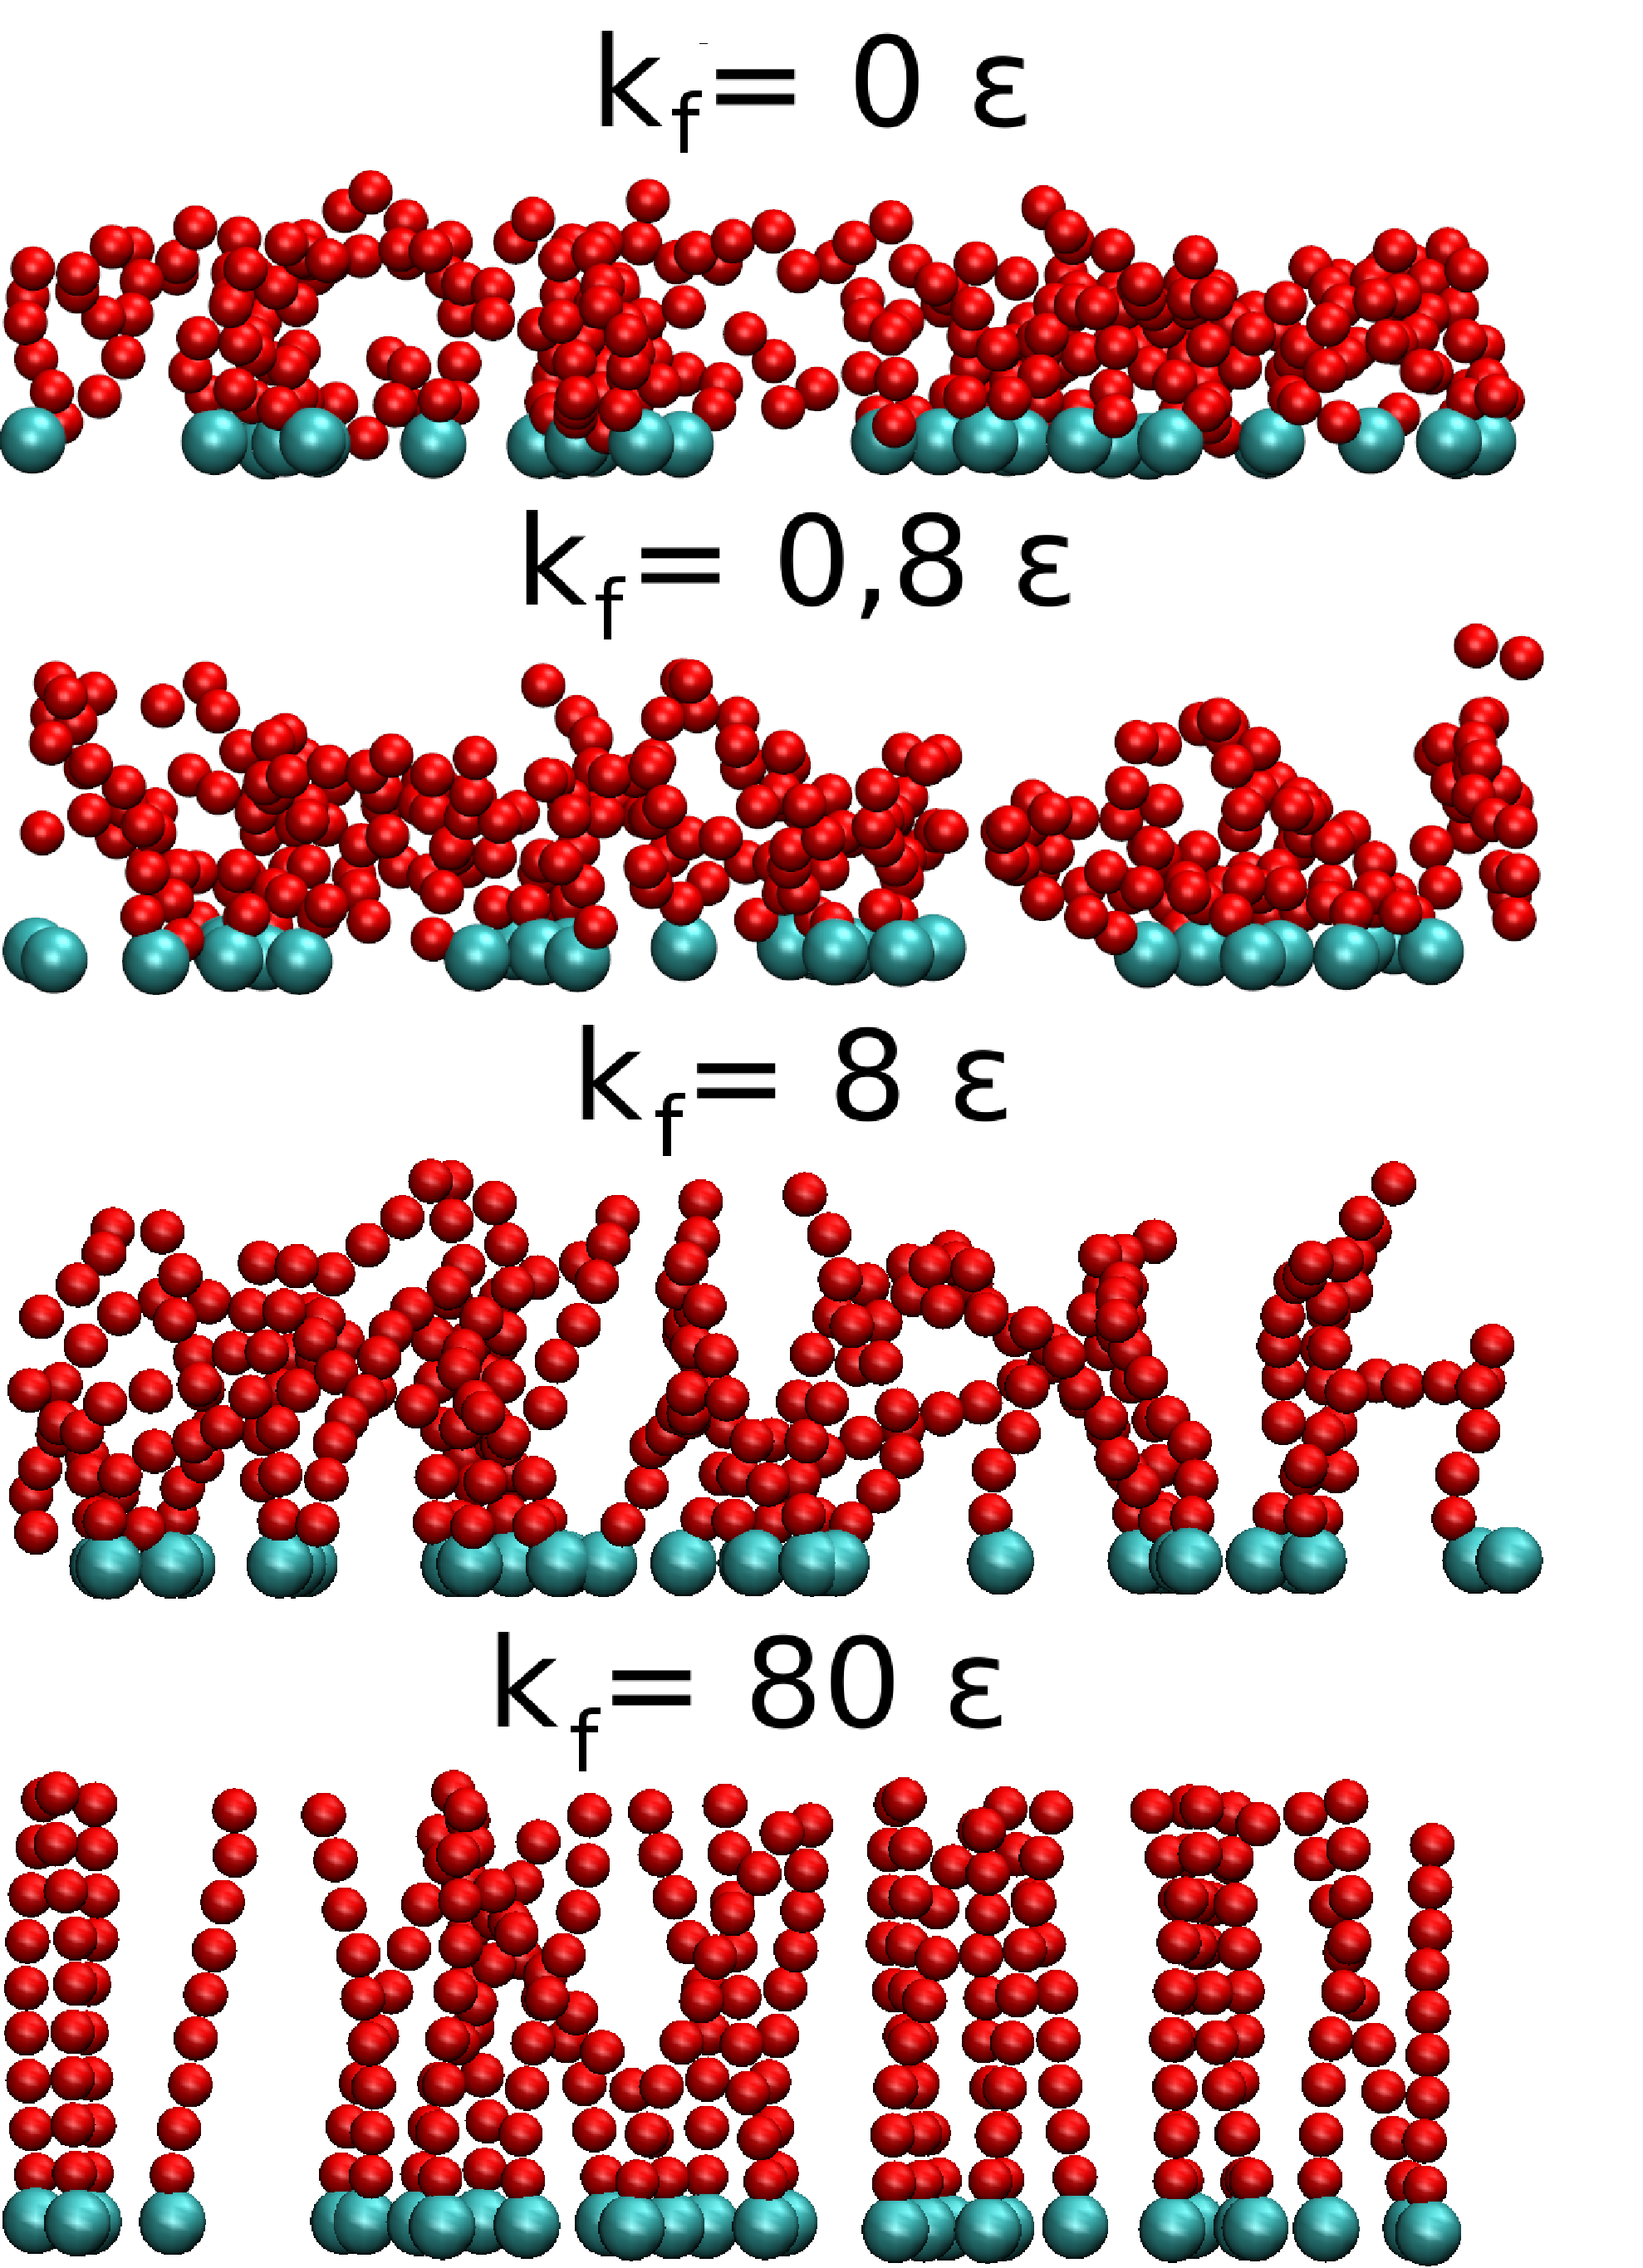
\includegraphics[clip,width=0.26\columnwidth]{figs/Brushes2}  & 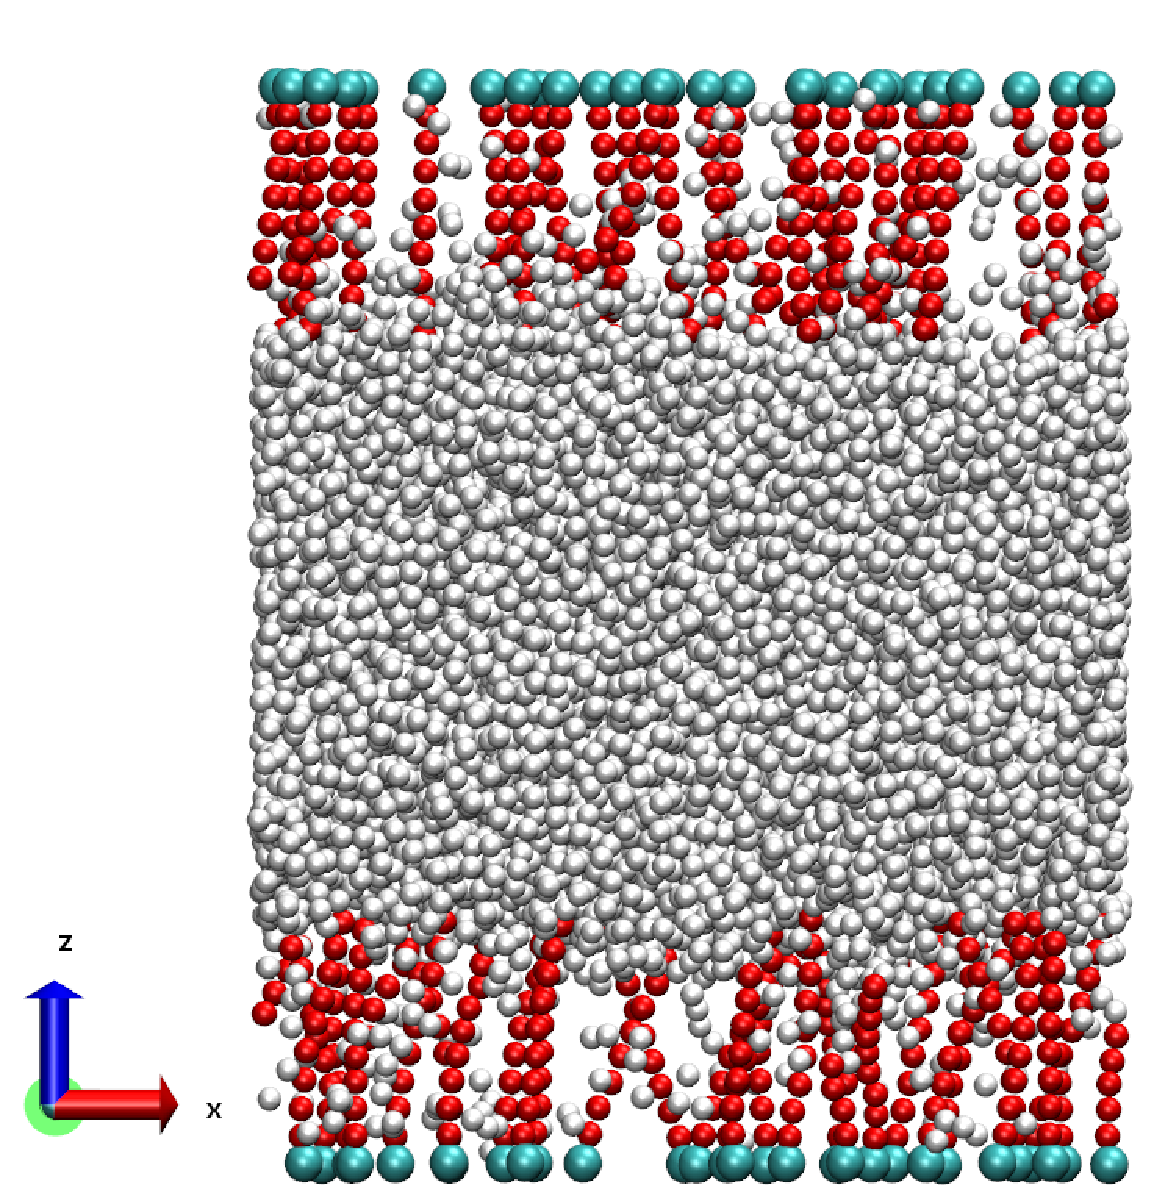
\includegraphics[clip,width=0.28\columnwidth]{figs/Muestra1}  & 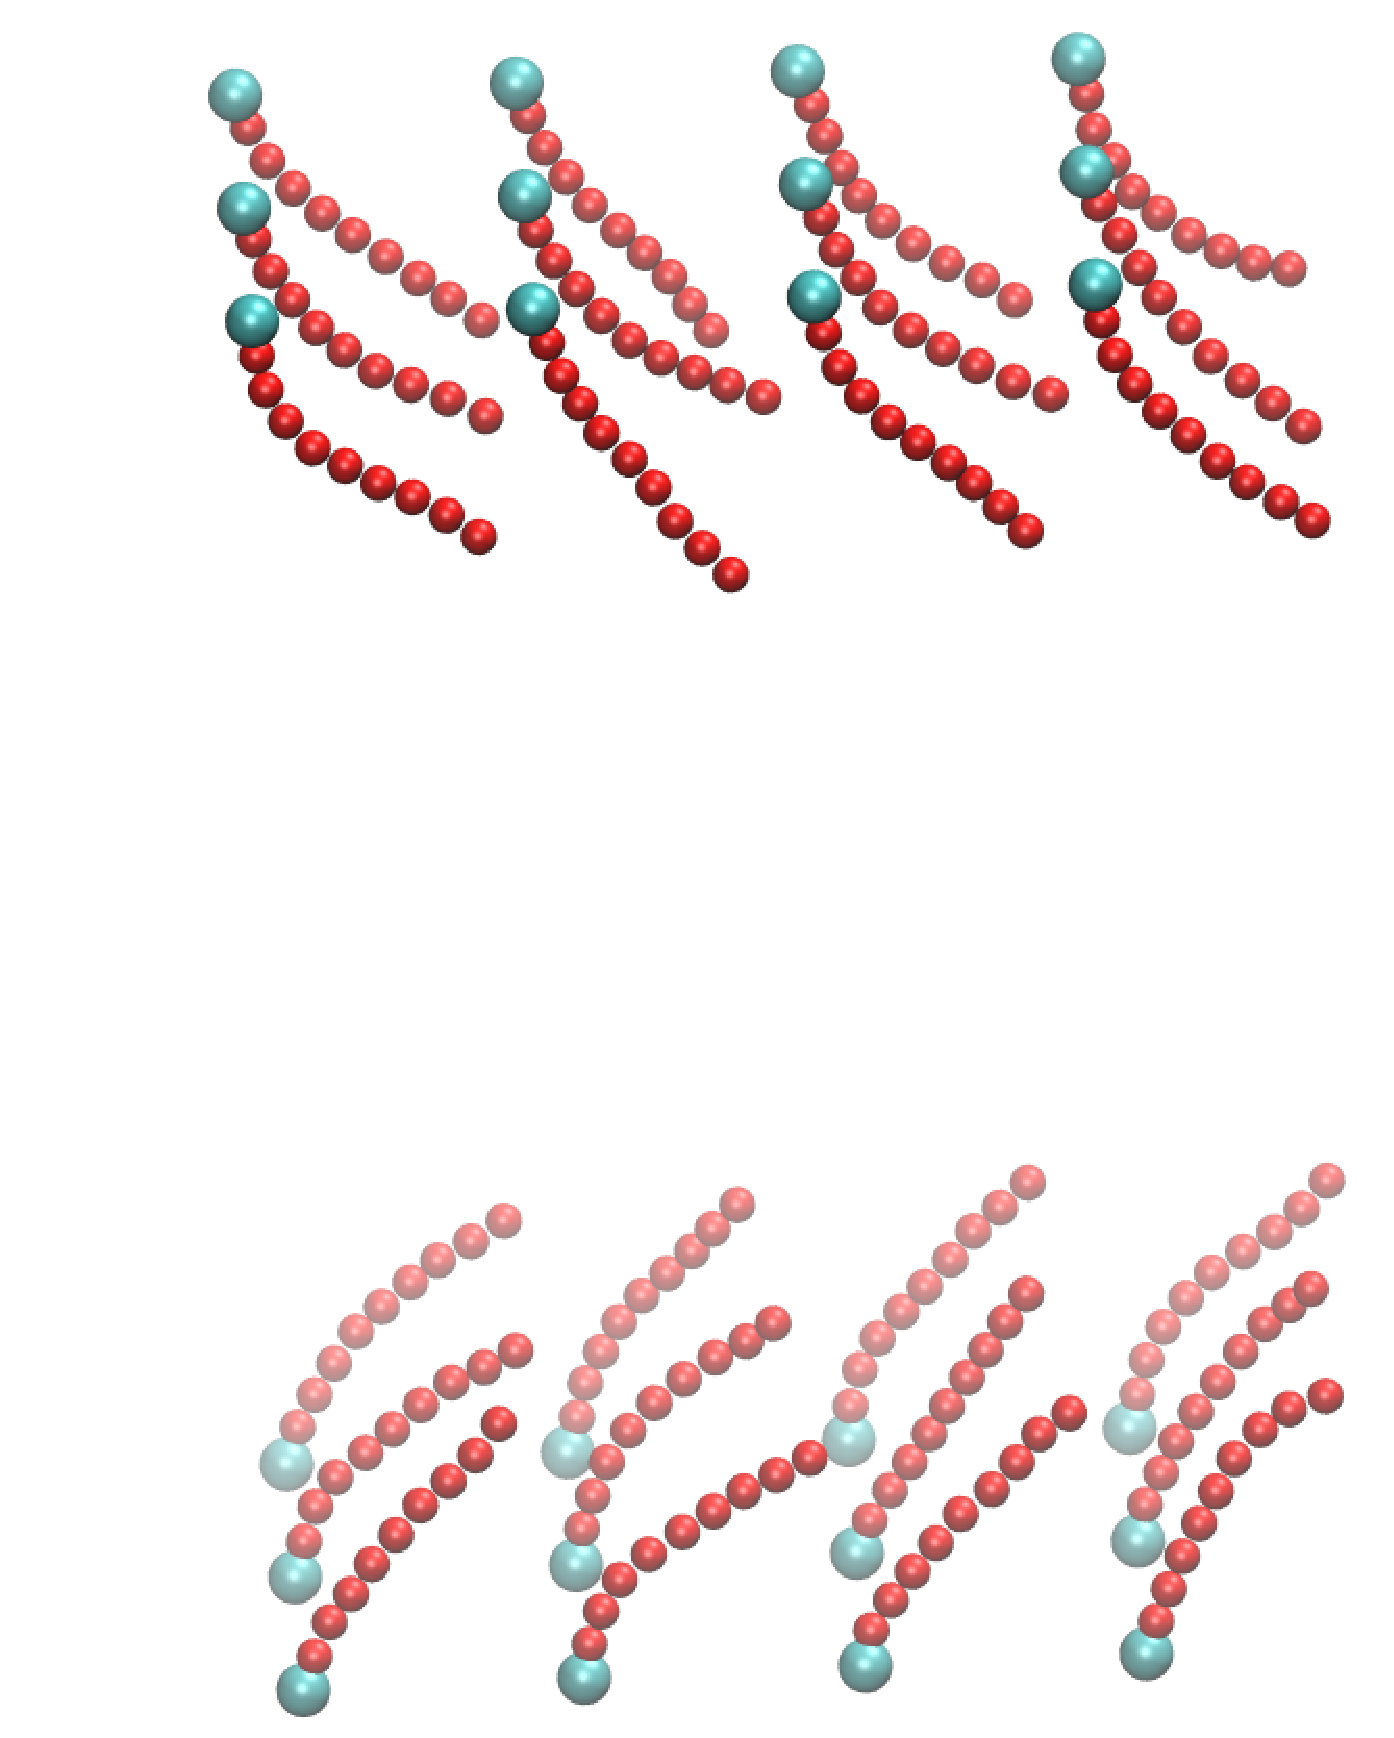
\includegraphics[clip,width=0.28\columnwidth]{figs/active_brush}\tabularnewline
\end{tabular}
\par\end{centering}

\protect\caption{Left panel: Grafted polymer layers with increasing stiffness, which
is parameterized by the bending constant $k_{f}$. Center panel: Planar
channel filled with liquid confined between two stiff polymer brush
layers with $k_{f}=80$. Right panel: Illustration of an active brush
oscillating with the same phase (phase-locked state, grafting points
arranged on square lattice). \label{fig_brushes} }
\end{figure}



A preliminary feasibility study that illustrates this kind of driving in  our coarse-grained model of semiflexible brushes is presented in Fig.~\ref{fig_brushes}. The asymmetric beating pattern of the semiflexible polymers consists of a power stroke and a recovery stroke -- essential features of active, biological systems. In the former the cilium stretches out and moves rather fast in one direction. In the recovery stroke, in turn, the cilium bends and slowly retracts \cite{Elgeti_15}. 

This asymmetric motion results from an internal activity in biological cilia. In our project is driven by an external, periodic force that acts on the bottom part of the grafted polymers.  As a first step, we have begun to characterize the polymer motion in the absence of an explicit solvent, where there is no hydrodynamic coupling between grafted molecules. Neighboring brush molecules are only coupled via the direct steric interaction (i.e., chain molecules cannot cross through each other in the course of their motion) or, additionally, via a harmonic coupling of neighboring chains close to the grafting point. This very simple model already exhibits different behaviors as a function of the frequency of the driving forces, and details of the coupling between neighboring chains. Based on these promising results, we will immerse the brush in a simple liquid and study the collective dynamics and synchronization as well as the impact of the driving on the dynamics of the liquid.

During his two-month stay in G\"ottingen, Kevin Speyer will address the following specific questions: 
\begin{itemize}
\item What is the relative importance of mechanical/steric and hydrodynamic interactions in the collective dynamics and synchronization of the polymer chains? 
\item How can one optimize the asymmetric motion pattern of the semiflexible grafted polymers to produce a directed flow at the vicinity of the brush-liquid interface?
\end{itemize}
Having achieved an understanding of these two basic questions there are several extensions that could be pursued in the following, final year of Kevin Speyer's Ph.D. project. The specific selection depends of the outcome of the present project but two follow-up studies illustrate the potential of this new project.
\begin{itemize}
\item How does the externally driven motion of the brush coating affect the friction of the brush-coated surface. Can one tailor the friction properties by the external driving or can one impart an anisotropy?  
\item Methachronal waves are frequently observed in biological cilia, i.e., there are regions of perfect synchronization surrounded by disordered beating patterns. Can one observe similar features in externally driven systems?  
\end{itemize}


\subsection{\noindent Methodology}

In accord with Kevin Speyer's previous work, we will use molecular dynamics simulations of coarse-grained bead-spring models. The active polymer brushes are described by the Kremer-Grest model \cite{Grest_86,Kremer_90}, where segments interact via a Lennard-Jones potential describing the harsh excluded volume of individual segments. A Finite Non-linear Extensively Elastic (FENE) potential accounts for the chain connectivity. We have used this model in our previous joint work on polymer brushes \cite{Pastorino_06,Pastorino_09,Pastorino_14}. Additionally, we apply a harmonic bending potential between two consecutive bonds that connect a given monomer with its two nearest neighbors in order to tune the rigidity of the semi-flexible polymer chain \cite{Speyer_15}.

The applicant has significant experience in the study of semi-flexible brushes under flow and has implemented the bending potential in the self-written, MPI-parallel  molecular dynamics program \cite{Speyer_15,doi:10.1021/acs.langmuir.7b02640}. Importantly, the combination of harsh excluded-volume interactions between segments and a maximal bond length guarantees that chain contours cannot cross through each other in the course of the simulation \cite{Grest_86,Kremer_90}. These entanglement effects that dramatically alter the dynamics in dense melts of long polymers are expected to be important for the synchronization of the active polymers.

We are planning the use of molecular dynamics simulation with a DPD (or Lowe-Anderson) thermostat \cite{DPD1,Lowe}. This pairwise thermostat obeys translation invariance and locally conserves momentum, thereby duly accounting for hydrodynamic interactions that are mediated via the explicit solvent \cite{Mueller_09,Pastorino_07,Pastorino_15}. We have experience in using this simulation techniques to study isothermal flows in nano-channels \cite{Mueller_08b,Pastorino_15,Pastorino_14,Leonforte_11}.

The MPI-parallel simulation code of the Argentine group is well suited for computer clusters; in G\"ottingen, the applicant will have additionally the opportunity to learn the use and programming of a GPU-program that is based on the HOOMD code (see http://glotzerlab.engin.umich.edu/hoomd-blue).
%%CP: does not compile refs properly
%%\footnote{\url{http://glotzerlab.engin.umich.edu/hoomd-blue}}
The latter allows for large-scale simulations on clusters of GPUs that are available at the von-Neumann Institute for Computing (NIC) in J\"ulich. This transfer of knowledge will be beneficial for the Argentine group because of the availability of computational resources in  G\"ottingen and the very good performance-to-price ratio of GPUs. Additionally, the research stay in G\"ottingen will offer opportunities to interact with the members of the SFB 937 \textquotedblleft Collective behavior of soft and biological matter \textquotedblright{}, in particular the group of J\"org Enderlein (III Institute of Physics) and Eberhard Bodenschatz (MPI for dynamics and self-organization).  


\section{Detailed work plan}
\begin{itemize}
\item Channel with explicit solvent: synchronization and hydrodynamic coupling

\begin{itemize}
\item An explicit solvent will be added to channels coated by active brushes,
described by Lennard-Jones particles, to account for momentum conservation
and the concomitant hydrodynamic interactions, taking advantage of
the experience of the German group. 
\item We will analyze the effect of solvent-mediated hydrodynamic coupling
between active chains and characterize changes in the collective chain
dynamics, as compared to the case of elastic coupling alone (in dry
brushes). 
\end{itemize}
\item Liquid flow with synchronized chain dynamics

\begin{itemize}
\item Imposing coordinated movement to the chains, mimicking typical cilia
dynamics, we will study the flow generated in the solvent. 
\item Upper and lower active brush layers of the slit channel will be studied
as a function of polymer beating frequency, amplitude, and direction.
Directed flow in the vicinity of the individual active brush layers
can be achieved by choosing parameters that result in synchronization
 or by
imposing a phase-locked dynamics with a time-dependent external force. 
\item Special interesting cases are in-phase movement of active upper and
lower brushes and anti-phase movement of upper and lower grafted layers.
If the polymers drive locally the fluid, the in-phase movement is
expected to produce a plug flow, whereas the anti-phase movement results
in shear flow. 
\item A parallelization scheme with GPU of some parts of the code will be
studied and implemented by the applicant with the help of the Prof.
M\"uller and his group. 
\end{itemize}
\end{itemize}
%\bibliographystyle{plain}
\bibliographystyle{unsrt}
%\bibliographystyle{apsrev}
\bibliography{biblio,c_refs,bibtex}

\end{document}
